\chapter{Исследовательский раздел}

\section{Цель исследования}

Целью исследования является анализ влияния размера личной колоды игрока и
используемой структуры хранения данных на производительность операций
завершения хода и формирования новой руки игрока.

В рамках исследования сравнивались структуры данных
\texttt{list}~\cite{py-list} и
\texttt{deque}~\cite{py-deque},
используемые для хранения игровых колод. Также оценивалось влияние
необходимости
перемешивания сброса на общее время выполнения операций.

\section{Методика проведения исследования}

Для проведения исследования была реализована программа, моделирующая завершение
хода игрока.

Во время выполнения операции выполнялись следующие шаги:

\begin{enumerate}
	\item перенос карт из руки игрока в сброс;
	\item перенос карт из сброса обратно в колоду добора;
	\item перемешивание колоды;
	\item добор новой руки.
\end{enumerate}

Исследование проводилось для двух вариантов организации хранения колоды:

\begin{itemize}
	\item \texttt{list};
	\item \texttt{deque}.
\end{itemize}

Замеры выполнялись для колод различных размеров:

\begin{itemize}
	\item 20 карт;
	\item 50 карт;
	\item 100 карт;
	\item 200 карт;
	\item 500 карт;
	\item 1000 карт;
	\item 2000 карт.
\end{itemize}

Для уменьшения влияния случайных факторов каждый эксперимент повторялся 1000
раз, после чего вычислялось среднее время выполнения операции.

Дополнительно исследования выполнялись в двух режимах:

\begin{itemize}
	\item без перемешивания сброса;
	\item с перемешиванием сброса.
\end{itemize}

Время выполнения измерялось с использованием функции \texttt{perf\_counter()}
языка Python.

\section{Результаты исследования}

В ходе исследования были построены графики зависимости времени выполнения
операции завершения хода от размера колоды. Графики представлены на
рисунках~\ref{img:full},~\ref{img:small}.

\begin{figure}[H]
	\centering
	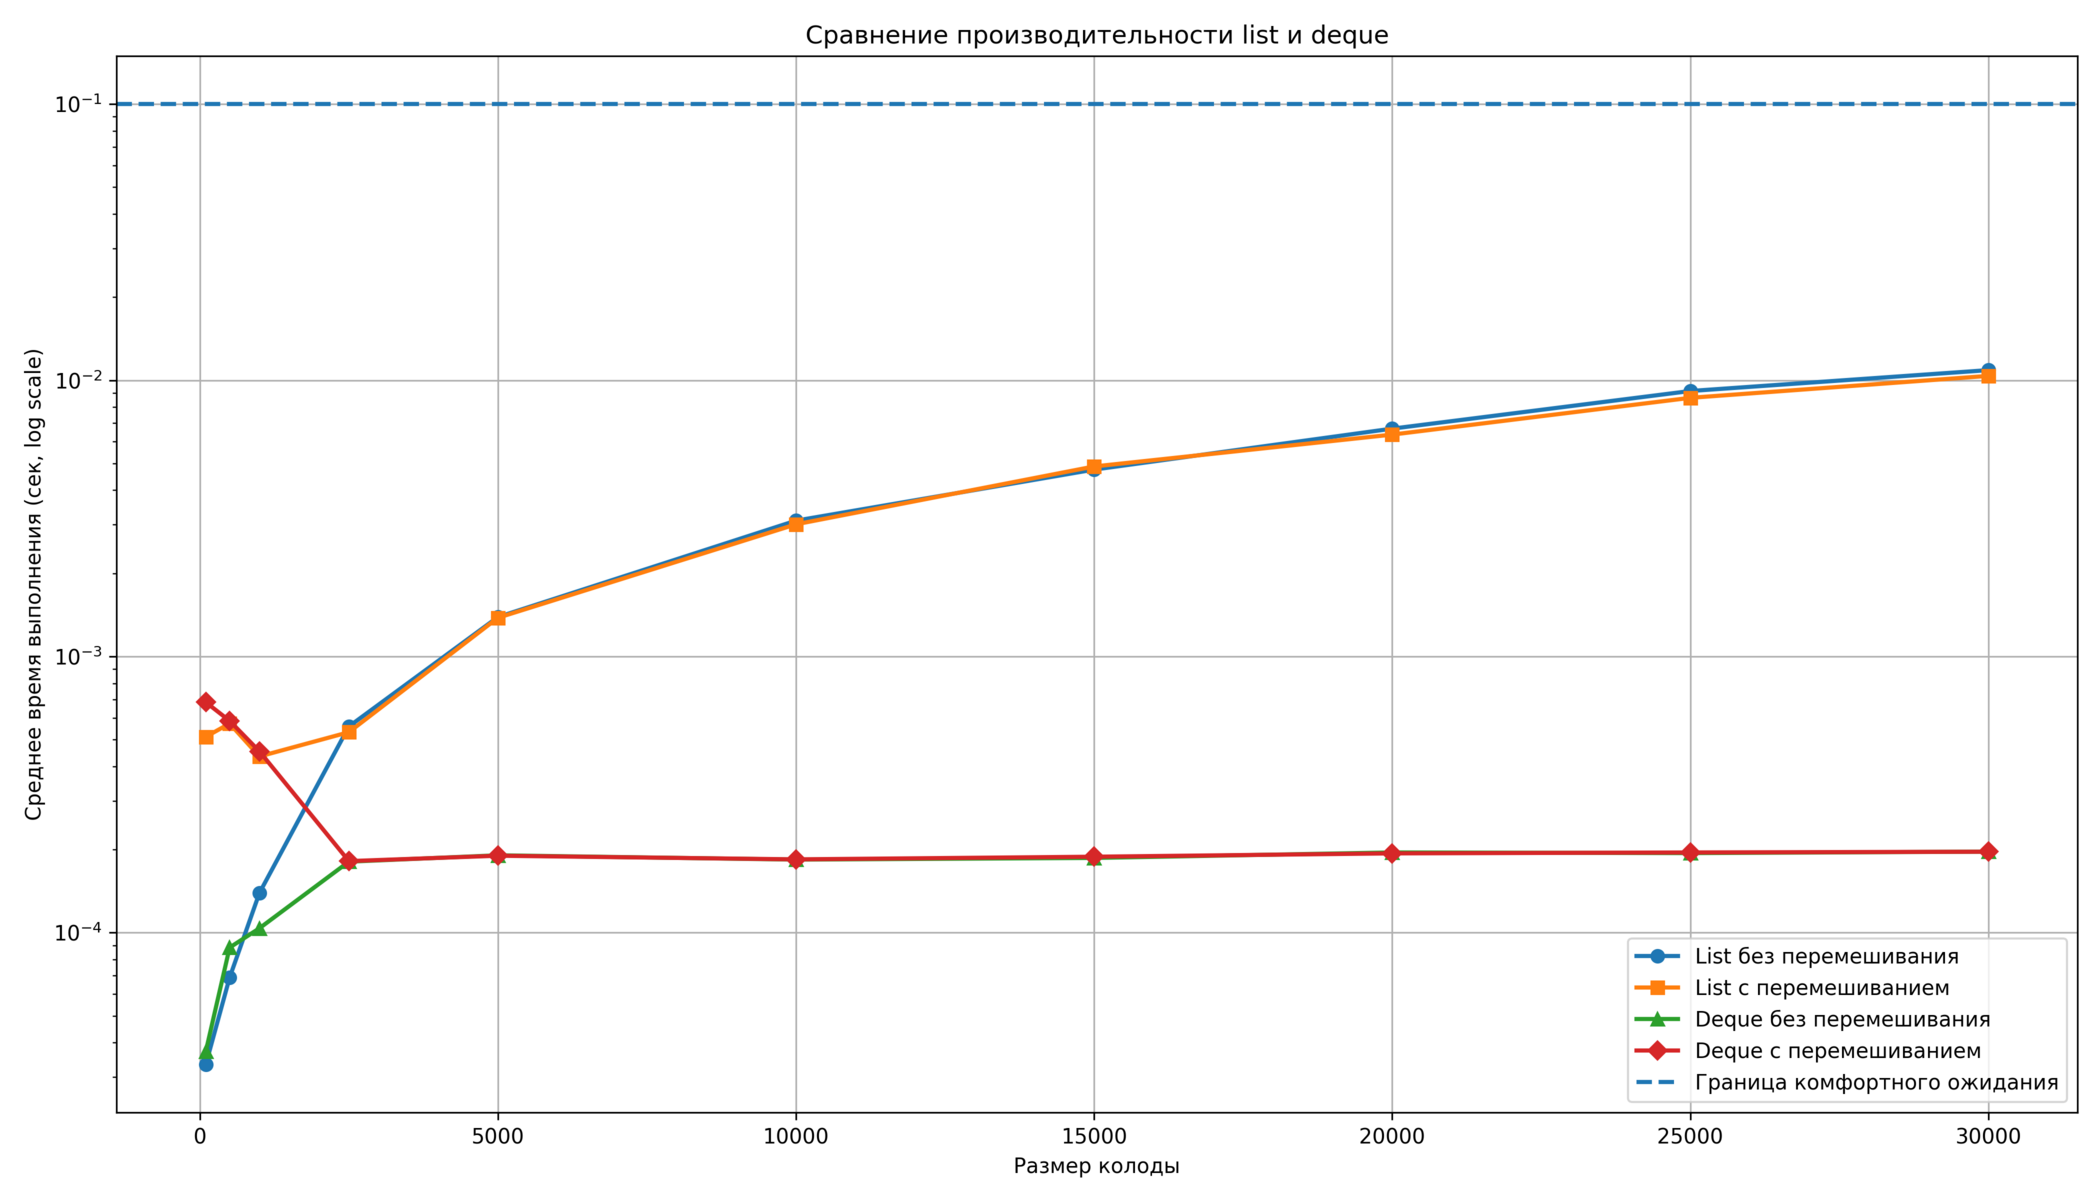
\includegraphics[width=0.9\linewidth]{../img/deck_performance_full}
	\caption{График замеров времени формирования колоды с временем
		комфортного ожидания пользователя}
	\label{img:full}
\end{figure}

\begin{figure}[H]
	\centering
	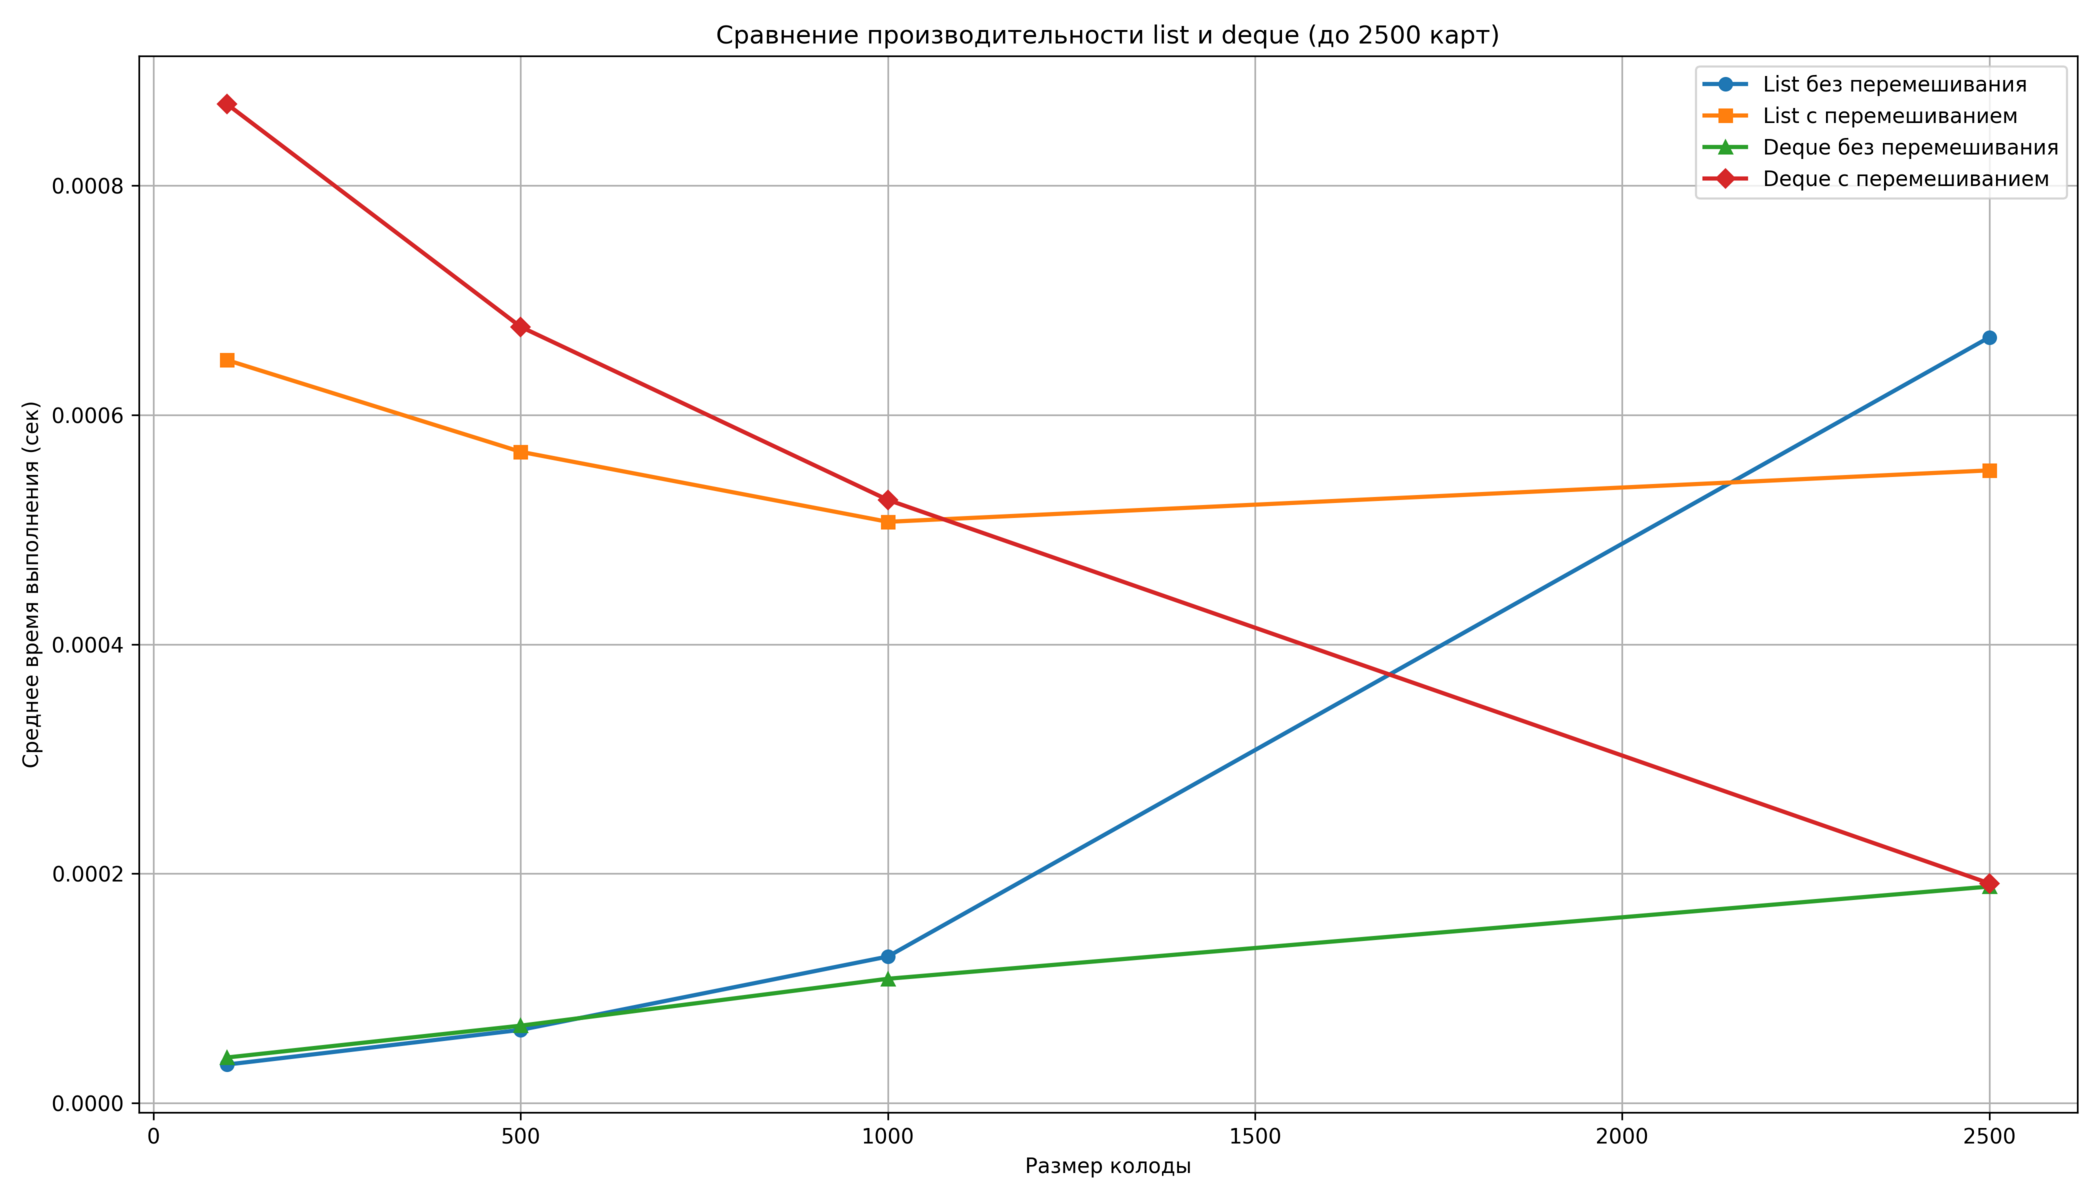
\includegraphics[width=0.9\linewidth]{../img/deck_performance_small}
	\caption{График замеров времени формирования колоды на малых значениях}
	\label{img:small}
\end{figure}

Результаты показали, что:

\begin{itemize}
	\item время выполнения операций увеличивается с ростом размера колоды;
	\item необходимость перемешивания оказывает значительно большее влияние
	      на
	      производительность, чем сам размер колоды;
	\item структура \texttt{list} демонстрирует более высокую
	      производительность при
	      отсутствии перемешивания;
	\item при использовании перемешивания различия между \texttt{list} и
	      \texttt{deque}
	      уменьшаются из-за дополнительных затрат на перестановку
	      элементов.
\end{itemize}

Также было установлено, что основное время выполнения затрачивается на операции
копирования и перемешивания элементов колоды.

\section*{Вывод}

В результате исследования было установлено, что производительность игровых
операций зависит не только от размера колоды, но и от используемой структуры
хранения данных, а также от необходимости перемешивания сброса.

Для операций последовательного хранения и добора карт структура \texttt{list}
показала более высокую производительность. Однако при частых операциях удаления
элементов из начала коллекции использование \texttt{deque} позволяет уменьшить
накладные расходы.

Наибольшее влияние на время выполнения оказывает операция перемешивания колоды,
поскольку она требует обработки всех элементов коллекции.
